\documentclass[11pt]{article}

\usepackage{titling,lipsum}
\usepackage[margin=1.5in]{geometry}
\usepackage{graphicx,amsmath,hyperref}
\usepackage[english]{babel}
\usepackage[utf8]{inputenc}
\usepackage{fancyhdr}

\newenvironment{localsize}[1]
{%
  \clearpage
  \let\orignewcommand\newcommand
  \let\newcommand\renewcommand
  \makeatletter
  \input{bk#1.clo}%
  \makeatother
  \let\newcommand\orignewcommand
}
{%
  \clearpage
}

\pagestyle{fancy}
\fancyhf{}
\rhead{ENGN3100 Report}
\lhead{Uri Pierre Burmester (u5561093)}
\rfoot{Page \thepage}

\title{ENGN3100 Practical Experience Report}
\author{Uri Pierre Burmester (u5561093)}
\date{\today}

\begin{document}

\begin{figure} \centering
  
\includegraphics[width=0.5\linewidth]{ANU.png}
\end{figure}

\maketitle

\centerline{AUSTRALIAN NATIONAL UNIVERSITY}  
\centerline{College of Engineering and Computer Science} 

\bigskip

\centerline{This Report is submitted in partial fulfilment of the Requirements for Practical Experience}
\centerline{ for the BE Degree in the ANU College of Engineering \& Computer Science}

\newpage

\tableofcontents

\newpage

\section{Summary of Practical Experience}

Period 1: \\
Name of Employer: Advanced Instrumentation and Technology Centre (AITC) \\
Starting date of Employment: 20/11/2017 \\
Ending date of Employment: 19/01/2018 \\
Position/job: Summer Research Intern - High-altitude Balloon Project \\
Weeks of experience claimed: 8 \\

\medskip

Period 2: \\
Name of Employer: Questacon - The National Science and Technology Centre \\
Starting date of Employment: 01/08/2017 \\
Ending date of Employment: 19/11/2017 \\
Position/job: Gallery Assistant \\
Weeks of experience claimed: 4 \\

Total number of weeks of experience claimed: 12

\newpage

\section{Employment Letters / Declaration of requirements}
\subsection{AITC Letter}

\begin{figure}[!h] \centering
  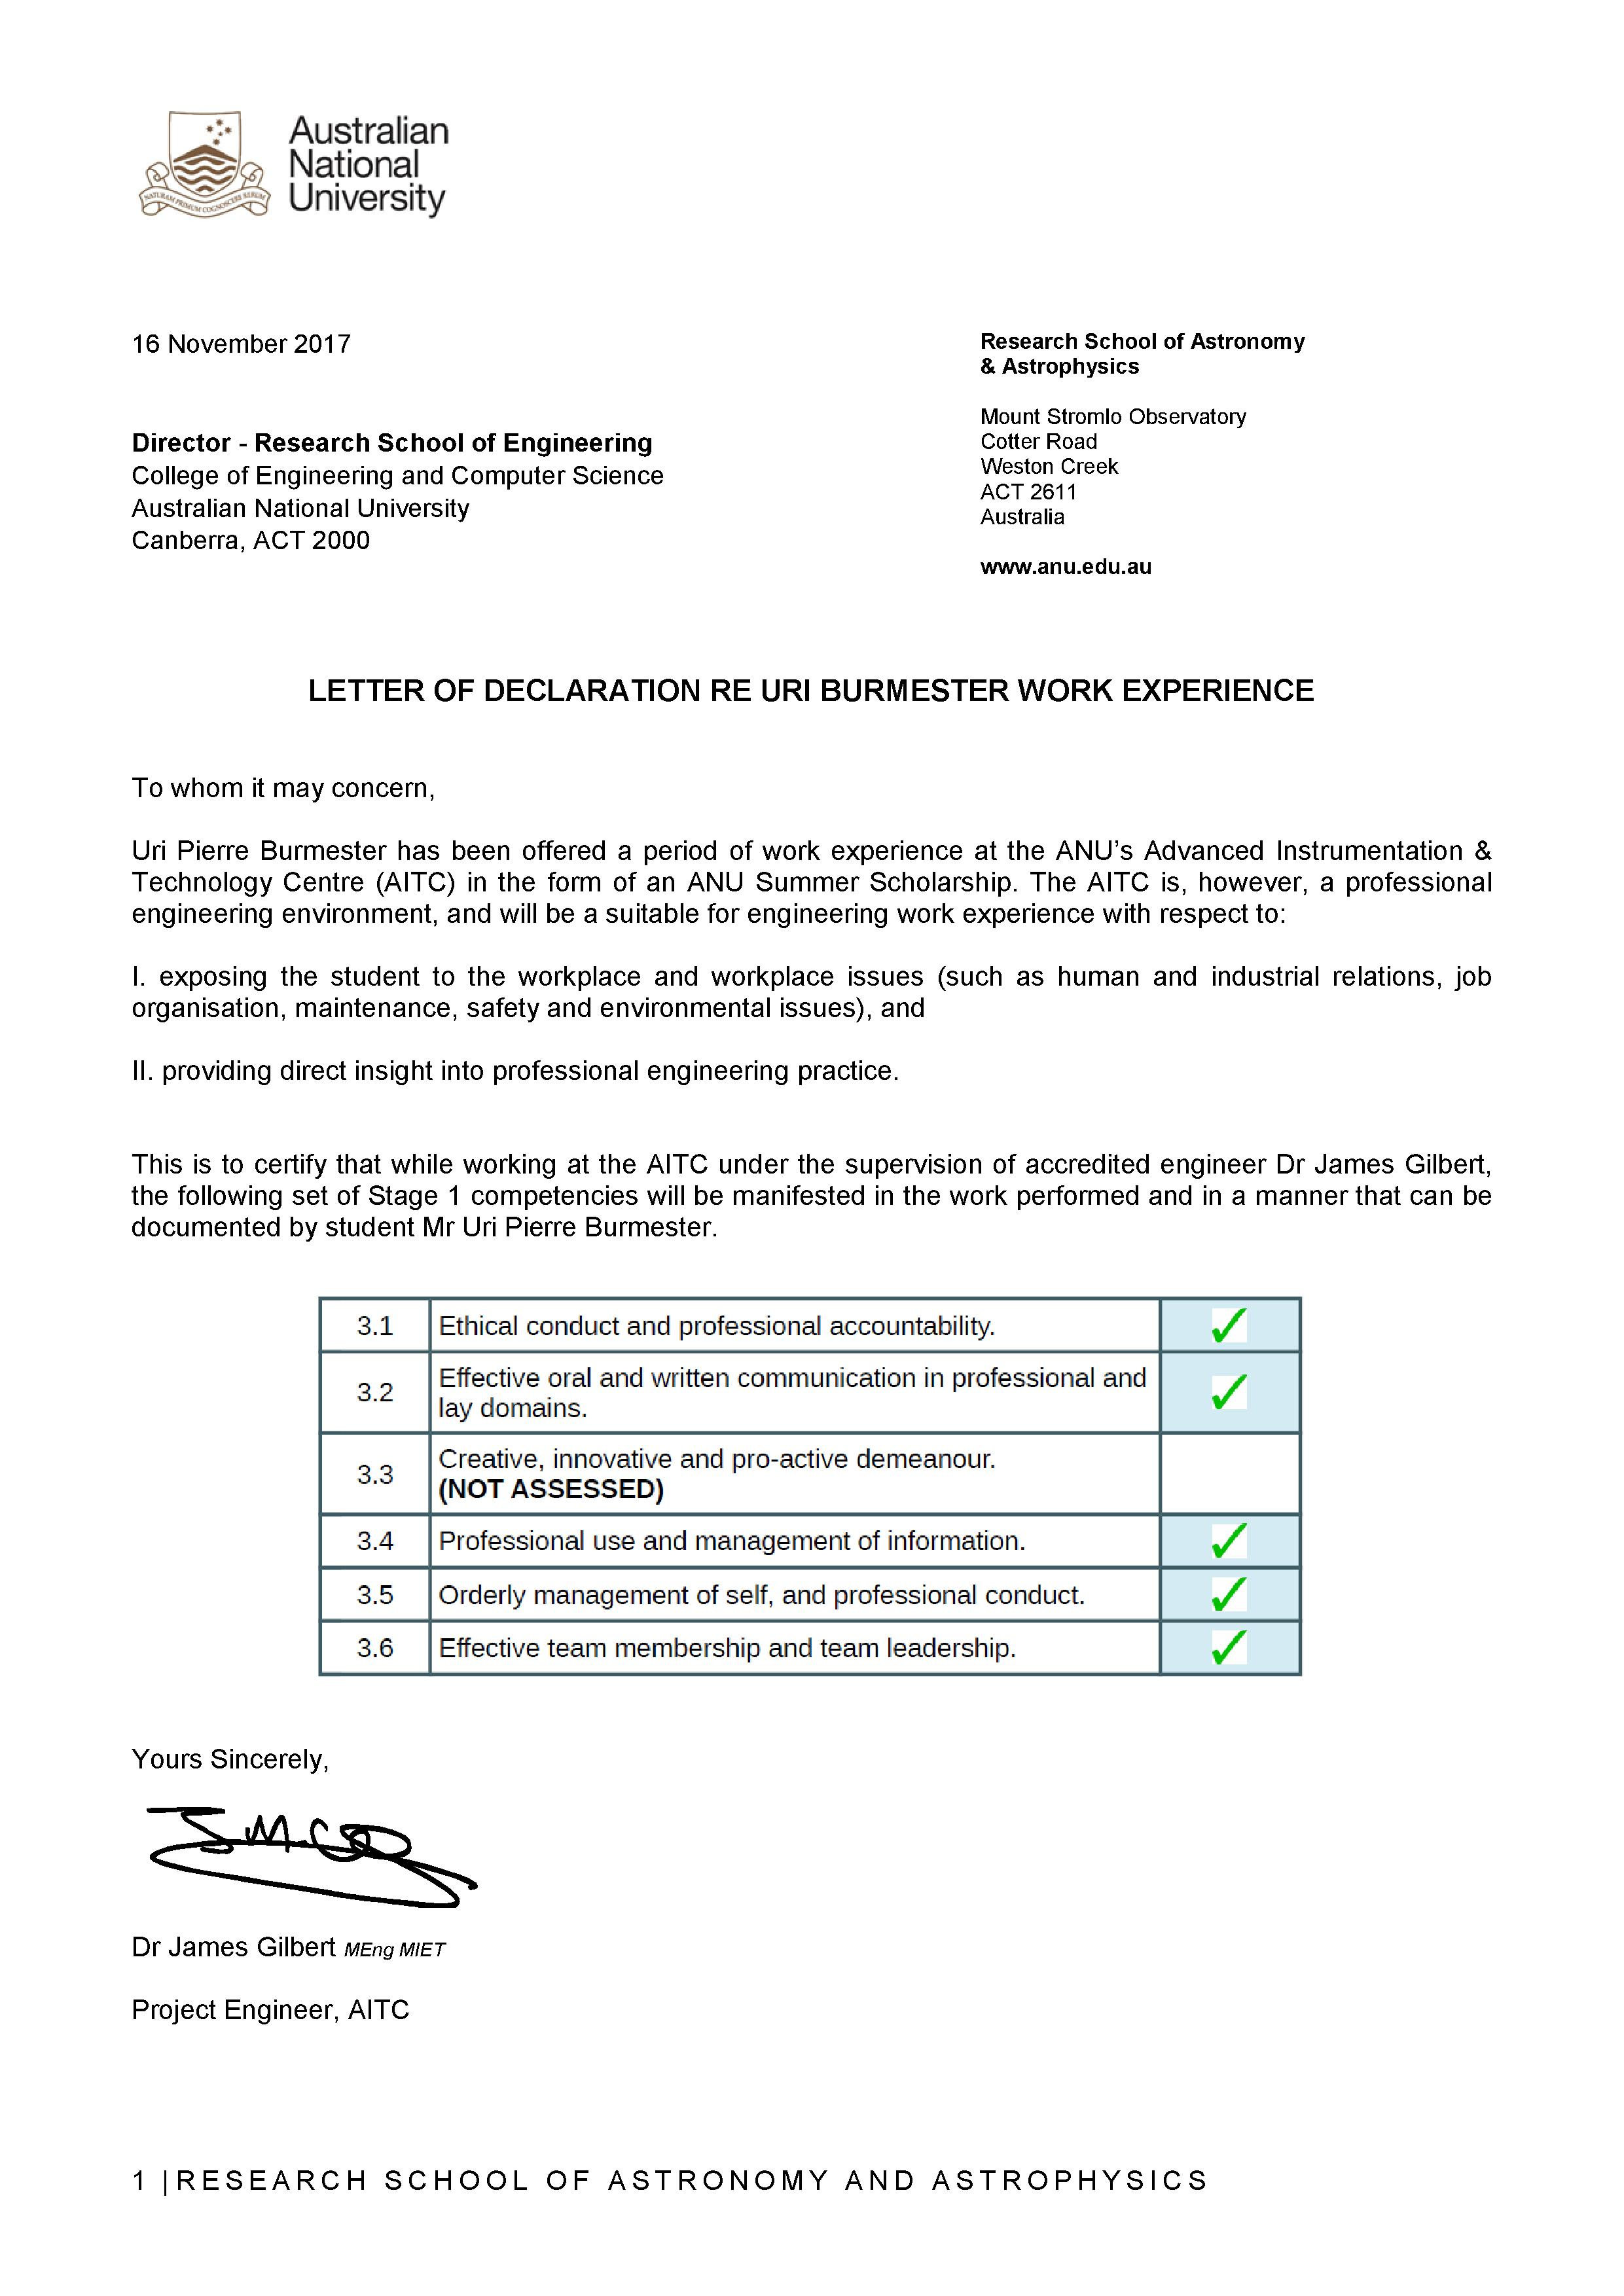
\includegraphics[width=0.9\linewidth]{upb_offer-signed.jpg}
\end{figure}

\newpage

\subsection{Questacon Letter}

SIGNED LETTER OF EMPLOYMENT FROM QUESTACON

\newpage

\section{Report}

\subsection{AITC Report}

\subsubsection{The structure and operation of the company}
-3-4 pages

The Advanced Instrumentation Technology Centre, located on the Mount Stromlo Observatory complex is run by the Australian National University's (ANU's) Research School of Astronomy and Astrophysics. Being part of the aerospace industry in Australia, the AITC has a great deal of corporate and research partners in Australia and internationally. Some of these include:

\begin{itemize}

\item Giant Magellan Telescope

\item CAASTRO: Centre of Excellence for All-Sky Astrophysics

\item Electro Optic Systems (EOS)

\item Gemini Observatory

\item Planetary Science Institute (PSI)

\item Space Environment Research Centre (SERC)

\item Harvard/Smithsonian \& Max Planck Institute for Astronomy

\item ANU Research School of Earth Sciences

\item ANU Research School of Physics and Engineering 

\item ViPAC Engineers \& Scientists

\item Smithsonian National Air \& Space Museum

\item Australian Astronomical Observatory

\end{itemize}

Full contact details for the AITC and its Head of Division are listed below in tables 1 and 2.

\begin{table}[!h] \centering 
 \label{contact} 
 \begin{tabular}{|c  c |} 
 \hline
 \multicolumn{2}{|l|}{Contact Details:} \\
   & \\
 T & +61 2 6125 0230 \\
 E & aitc@anu.edu.au \\
 W & aitc.anu.edu.au \\
   & \\
 \multicolumn{2}{|l|}{Advanced Instrumentation and Technology Centre} \\
 \multicolumn{2}{|l|}{Mount Stromlo Obervatory, Weston ACT 2611} \\
  \hline
   \end{tabular}
\caption{AITC Contact Details}
\end{table}

\begin{table}[!h] \centering 
 \label{moore}
 \begin{tabular}{|c  c |} 
 \hline
  \multicolumn{2}{|l|}{Professor Anna Moore} \\
   & \\
 T & +61 2 6125 4724 \\
 E & Anna.Moore@anu.edu.au \\
   & \\
 \multicolumn{2}{|l|}{Commonwealth Solar Observatory, Admin Wing} \\
 \multicolumn{2}{|l|}{Mount Stromlo Obervatory, Weston ACT 2611} \\
   \hline
   \end{tabular}
\caption{Professor Anna Moore Contact Details}
\end{table}



- Managerial and administrative structure of the company.
- Company's business/ products, production output, trading partners, markets.
- Company's divisions (if there are any). Division's business/products, etc.
- Name and address of the Head of the Division.
- Company's financial base, is it private or public, is it listed on Stock Exchange?
- Total operation budget, division into business areas.
- Attitude of the company to its work-force, prevailing ethics in the company.

\newpage

\subsubsection{My Position in the Company}
My position at the AITC was as a "Summer Research Intern". My immediate supervisor was Dr. Jamie Gilbert and, as one of his interns, my work was restricted to the scope of Dr. Gilbert's High-Altitude Balloon (HAB) project.As a Project Engineer in the AITC, Dr. Gilbert then reported directly to Dr. Anna Moore. \\ 

My role at the AITC was mostly focused on the HAB project, to write a software framework to predict the landing sites of HABs. It was my responsibility to set my own project scope and deadlines. I conducted my own research into the topic and implemented the code based on my research. I made regular reports to Dr. Gilbert about my progress on the project and implemented his feedback. It was also my responsibility to aid Dr. Gilbert with tasks relating to the balloon launch, including assembling the payload, filling the balloon and retrieving the payload after the flight. \\ 

The main interaction with other employees was with the other Summer Interns - many of us would confer on the details of the projects that we were conducting in order to share knowledge and expertise. This mainly took the form of informal meetings over lunch, afternoon tea or at our desks. For example, we would share ideas regarding how to program certain processes in software, possible sources of errors in our results and whether or not our work was on the right track. Another point of contact was with Prof. Celine D'Orgeville, who was the contact for students undertaking the Internship - she listened to my concerns about my own work as well as answering logistical questions about the structure and layout of the AITC. \\

I believe this job was offered to me because of my engineering project experience, my prior experiences in the workforce and my physics/astrophysics knowledge. As an engineering student at the ANU, I already had prior experience managing large-scale systems engineering projects - in particular, my education focused on the ability to break down large problems into more manageable parts, talk with a client and establish a system scope, requirements and deadlines. The extra research I've done into other project management techniques (e.g. Kanban, Scrum, agile) also likely worked in my favour as a candidate. Secondly, I believe that my time in the workforce contributed to the decision to hire me in particular. A candidate with similar knowledge to myself but with no experience working a steady job would be less familiar with the protocol of the workplace (e.g. email ettiquette, Workplace Health and Safety). Working a job in the past is also evidence of my ability to participate well in the workforce and act as an effective team member. Thus, I believe my previous time in the workforce was one of the reasons I was selected. Lastly, I believe that the courses I've taken in Physics and Astrophysics contributed to my being offered this position - taking these courses ensured that I was knowledgeable enough to understand the purpose behind the high-altitude balloon project and the physics underlying the flight. \\

\subsubsection{Technical Description of the Job}
-5-6 pages

During the employment, Uri’s job involved conducting a long-term, supervised engineering project to predict the landing sites of High-Altitude Balloons (HABs). This involved investigating customer needs in order to identify an appropriate scope, project requirements and deadlines, as well as implementing feedback throughout the project development process. Uri first conducted a literature review of the scientific and engineering principles underlying the project and then began writing a framework in software to handle the appropriate data. Uri constructed a framework to test the accuracy of his prototype code and then conducted further refinements of the design. Towards the end of the project, Uri made a formal presentation of his findings to stakeholders and industry partners (including the Space Environment Research Centre and EOS Space Systems), engaging them by answering question. Uri also wrote a formal engineering report of his findings which provided him with the opportunity to formally document his work, evaluate its strengths and weaknesses and identify areas for further development. During his time, Uri also participated in other aspects of the HAB project, including the construction of parts of balloon payload and assisting with the logistics of the balloon launch. 

- What I did (attach summary results as appendix, if relevant).
- What I achieved (attach any drawings, photographs, sketches as appendix, if
relevant).
- How did my work relate to Company's business?

\subsection{Questacon Report}

This report does not include my experiences at Questacon because, as stated in the requirements on the \href{http://programsandcourses.anu.edu.au/course/engn3100}{ENGN3100 course page}: "The report itself need only describe the experience at one of the places (must be one of the places satisfying the engineering requirement)."

\newpage

\section{Development of Stage 1 Competency Standards for Professional Engineer}

-2-3 pages
- How my experiences helped me work towards the standards of a
professional engineer.
- The standards identified by Engineers Australia are listed on the ENGN3100
WebCT report site
- Which areas of competency were developed, and how.\
PLEASE NUMBER EACH COMPETENCY CLAIMED ACCORDING TO THE
NUMBERING SYSTEM OF APPENDIX 1.


3 PROFESSIONAL AND PERSONAL ATTRIBUTES

ETHICAL CONDUCT AND PROFESSIONAL ACCOUNTABILITY (3.1):


EFFECTIVE ORAL AND WRITTEN COMMUNICATION IN PROFESSIONAL AND LAY DOMAINS (3.2):

PROFESSIONAL USE AND MANAGEMENT OF INFORMATION (3.4)


ORDERLY MANAGEMENT OF SELF, PROFESSIONAL CONDUCT (3.5)


EFFECTIVE TEAM MEMBERSHIP AND TEAM LEADERSHIP (3.6)


\newpage

\section{Employer Feedback Forms}

\subsection{AITC}

EMPLOYER FEEDBACK FORM FROM AITC

\newpage

\subsection{Questacon}

EMPLOYER FEEDBACK FORM FROM QUESTACON

\newpage

\section{Employer Declarations of Report Accuracy}

\subsection{AITC}

EMPLOYER DECLARATION FROM AITC

\newpage

\subsection{Questacon}

EMPLOYER DECLARATION FROM QUESTACON

\newpage

\section{Conclusions}
-1 page

\newpage

\section{Reflection of Work Experience}
The work experience process has been useful for me. The professional engineering context is very different from my experience of study and it was enlightening to observe these differences first-hand; in particular, I now have a concept of the professional skills required in the workplace and which of these skills I still need to develop in myself. The skills which I feel most need further development in myself include: \\

\begin{itemize}

\item Scheduling and Deadlines: Though I made great progress in combating this flaw during my time at the AITC, I believe there is still work to be done. Many times during this project, I found myself behind schedule and experiencing stress about how I would catch up to my proposed project timeline. Thus, I am going to make an effort in future projects to consult more with others and set more reasonable sub-deadlines to prevent myself from getting overwhelmed by work. 

\item Setting and sticking to an appropriate scope: I also felt that I was experiencing some scope creep during this project. At times, I looked at design decisions I'd make in software and realised that I'd make inadvertent assumptions about what my final product would look like that were not specified in the scope. In future, I'm going to attempt to be more "design agnostic" and talk to others to ensure I'm not setting an unrealistic (or changing) solution space.

\item Interacting Informally with Colleagues: I felt that in my time in the workforce, I did not make enough of an effort to get to know my colleagues outside of a professional context. Most of my interaction with my colleagues was purely business-related. However, there is more to the workplace than business - it can also be a place to make friends and build professional contacts that will be useful in later life. Thus, I am going to make an effort to further develop my social skills to be a better all-around member of the human community in the workplace rather than just a worker. 

\end{itemize}

\newpage

\section{Acknowledgements}

I would like to personally express my gratitude for my wonderful supervisor Dr. Jamie Gilbert. His insightful advice and positive attitude helped me every step of the way. \\

I would also like to acknowledge the help and support of Jess Brosnan from Questacon who has proven herself to be a friendly, helpful and supremely well-organised point-of-contact for me. I am very grateful for her support.\\

\section{Signature and date}

\medskip

Signature: .................................................................................................. \\
Date: \today

\newpage

\section{Appendix 1: Stage 1 Competency Matrix}

\begin{localsize}{10}

\begin{table}[!h] \centering
 \begin{tabular}{|p{0.75cm} | p{8cm} | p{1.5cm} | p{2cm} |} 
 \hline
  Unit & UNIT Descriptor & Claimed? [Y/N] & Section or Line or Paragraph in Report\\ \hline
   1 & KNOWLEDGE AND SKILL BASE & & \\ \hline
   1.1 & Comprehensive, theory based understanding of the underpinning natural and physical sciences and the engineering fundamentals applicable to the engineering discipline. & & \\ \hline
   1.2 & Conceptual understanding of the, mathematics, numerical analysis, statistics, and computer and information sciences which underpin the engineering discipline. & & \\ \hline
   1.3 & In-depth understanding of specialist bodies of knowledge within the engineering discipline. & & \\ \hline
   1.4 & Discernment of knowledge development and research directions within the
engineering discipline. & & \\ \hline
   1.5 & Knowledge of contextual factors impacting the
engineering discipline. & & \\ \hline
   1.6 & Understanding of the scope, principles, norms, accountabilities and bounds of contemporary engineering practice in the specific discipline. & & \\ \hline
   & & & \\ \hline
   2 & ENGINEERING APPLICATION ABILITY & & \\ \hline
   2.1 & Application of established engineering methods to complex engineering problem solving. & & \\ \hline
   2.2 & Fluent application of engineering techniques, tools and resources. & & \\ \hline
   2.3 & Application of systematic engineering synthesis and design processes & & \\ \hline
   2.4 & Application of systematic approaches to the conduct and management of engineering projects. & & \\ \hline
   & & & \\ \hline
   3 & PROFESSIONAL AND PERSONAL ATTRIBUTES & & \\ \hline
   3.1 & Ethical conduct and professional accountability & & \\ \hline
   3.2 & Effective oral and written communication in professional and lay domains & & \\ \hline
   3.3 & Creative, innovative and pro-active demeanour. & & \\ \hline
   3.4 & Professional use and management of information. & & \\ \hline
   3.5 & Orderly management of self, and professional conduct. & & \\ \hline
   3.6 & Effective team membership and team leadership. & & \\ \hline
   \end{tabular}  
\caption{Engineers Australia Competencies for Stage 1 Engineering Practitioners}
\end{table}

\end{localsize}

DEAD BITS

Based on my experiences working in the AITC and Questacon, I feel most confident in the following skills:

\begin{itemize}

\item Report writing: Having written many technical reports in a University setting in the past, I already felt confident in this skill. I understand the skills required to make a good technical report. In particular, I provide my reports with a sensible structure, I understand how to effectively typeset and cross-reference my work to allow the reader to understand my results and I understand how to document my choices and assumptions in a way that is accessible.

\item Presentation and communication: The presentation of my results at the end of my AITC internship was particularly helpful in refining my presentation and communication skills. For example, talking about a technical project with my fellow AITC interns challenged my ability to quickly explain the important points of a topic. Further, crafting a full presentation for my colleagues at the AITC and our corporate partners was a nerve-racking but ultimately rewarding experience. 

\item Research: Research is a skill that I employ in every University course that I undertake. It underlies my report on the HAB project and even my ability to effectively communicate with the guests at Questacon. I feel confident in my ability to research effectively by: scoping out information from a wide variety of sources, evaluating this information to understand its context, strengths and weaknesses and I understand how to cross-reference different sources to build up a strong chain of evidence. 

\end{itemize}

\end{document}